\section{Experiments}

We conduct extensive experiments on several large-scale image benchmark datasets to evaluate the performance of \texttt{HypStructure} as compared to the Flat and $\ell_2$-CPCC baselines for hierarchy embedding, classification, and OOD detection tasks. 


\label{sec:experiments}
\paragraph{Datasets and Setup}
Following the common benchmarks in the literature, we consider three real-world vision datasets, namely CIFAR10, CIFAR100~\citep{krizhevsky2009learning} and ImageNet100 \citep{ming2022delving} for training, which vary in scale, number of classes, and number of images per class. We construct the ImageNet100 dataset by sampling 100 classes from the ImageNet-1k \citep{imagenet} dataset following \citep{ming2022delving}. For CIFAR100, a three-level hierarchy is available with the dataset release \citep{krizhevsky2009learning}. Since no hierarchy is available for the CIFAR10 and ImageNet100 datasets, we construct a hierarchy for CIFAR10 manually in \Cref{fig:toy}. For ImageNet100, we create a subtree from the WordNet \citep{wordnet}  given 100 classes as leaves. More details regarding the datasets, network, training and setup are provided in the \Cref{app:exp_details_params}.


\subsection{Quality of Hierarchical Information}
\label{sec:tree_emb_quality}
\begin{figure*}[!ht]
    \centering
    \begin{minipage}{0.65\textwidth}
        \centering
        \captionof{table}{Evaluation of hierarchical information distortion and classification accuracy using \texttt{SupCon} \citep{2020supcon} as $\ell_\text{Flat}$. All metrics are reported as mean (standard deviation) over 3 seeds.}
        \resizebox{\textwidth}{!}{
            \begin{tabular}{lcccccccc}
                \toprule
                \multirow{2}{*}{\textbf{\begin{tabular}[c]{@{}c@{}}Dataset\\ (Backbone)\end{tabular}}} & \multirow{2}{*}{\textbf{Method}} & \multicolumn{2}{c}{\textbf{Distortion of Hierarchy}} & \multicolumn{2}{c}{\textbf{Classification Accuracy}} \\
                \cmidrule(lr){3-4} \cmidrule(lr){5-6}
                & & \textbf{$\delta_{rel}$ ($\downarrow$)} & \textbf{CPCC ($\uparrow$)} & \textbf{Fine ($\uparrow$)} & \textbf{Coarse ($\uparrow$)} \\
                \midrule
                \multirow{3}{*}{\begin{tabular}[c]{@{}c@{}}CIFAR10\\ (ResNet-18)\end{tabular}} & Flat & 0.232 (0.001) & 0.573 (0.002) & 94.64 (0.12) & 99.16 (0.04) \\
                & $\ell_2$-CPCC  & 0.174 (0.002) & 0.966 (0.001) & 94.47 (0.13) & 98.91 (0.02) \\
                & \cellcolor{gray!20}\texttt{HypStructure}  & \cellcolor{gray!20}\textbf{0.094 (0.003)} & \cellcolor{gray!20}\textbf{0.992 (0.001)} & \cellcolor{gray!20}\textbf{94.79 (0.14)} & \cellcolor{gray!20}\textbf{99.18 (0.04)} \\
                \midrule
                \multirow{3}{*}{\begin{tabular}[c]{@{}c@{}}CIFAR100\\ (ResNet-34)\end{tabular}} & Flat & 0.209 (0.002) & 0.534 (0.119) & 74.96 (0.14) & 84.15 (0.19) \\
                & $\ell_2$-CPCC  & 0.213 (0.006) & \textbf{0.779 (0.002)} & 76.07 (0.19) & 85.28 (0.32) \\
                & \cellcolor{gray!20}\texttt{HypStructure} & \cellcolor{gray!20}\textbf{0.127 (0.016)} & \cellcolor{gray!20}0.766 (0.007) & \cellcolor{gray!20}\textbf{76.68 (0.22)} & \cellcolor{gray!20}\textbf{86.01 (0.13)} \\
                \midrule
                \multirow{3}{*}{\begin{tabular}[c]{@{}c@{}}ImageNet100\\ (ResNet-34)\end{tabular}} & Flat & 0.168 (0.003) & 0.429 (0.002) & 90.01 (0.07) & 90.77 (0.11) \\
                & $\ell_2$-CPCC  & 0.213 (0.009) & 0.834 (0.002) & 89.57 (0.38) & 90.34 (0.28) \\
                & \cellcolor{gray!20}\texttt{HypStructure}  & \cellcolor{gray!20}\textbf{0.134 (0.001)} & \cellcolor{gray!20}\textbf{0.841 (0.001)} & \cellcolor{gray!20}\textbf{90.12 (0.01)} & \cellcolor{gray!20}\textbf{90.84 (0.02)} \\
                \bottomrule
            \end{tabular}
        }
        \label{tab:combined_metrics_accuracy}
    \end{minipage}
    \hfill
    \begin{minipage}{0.3\textwidth}
        \centering
        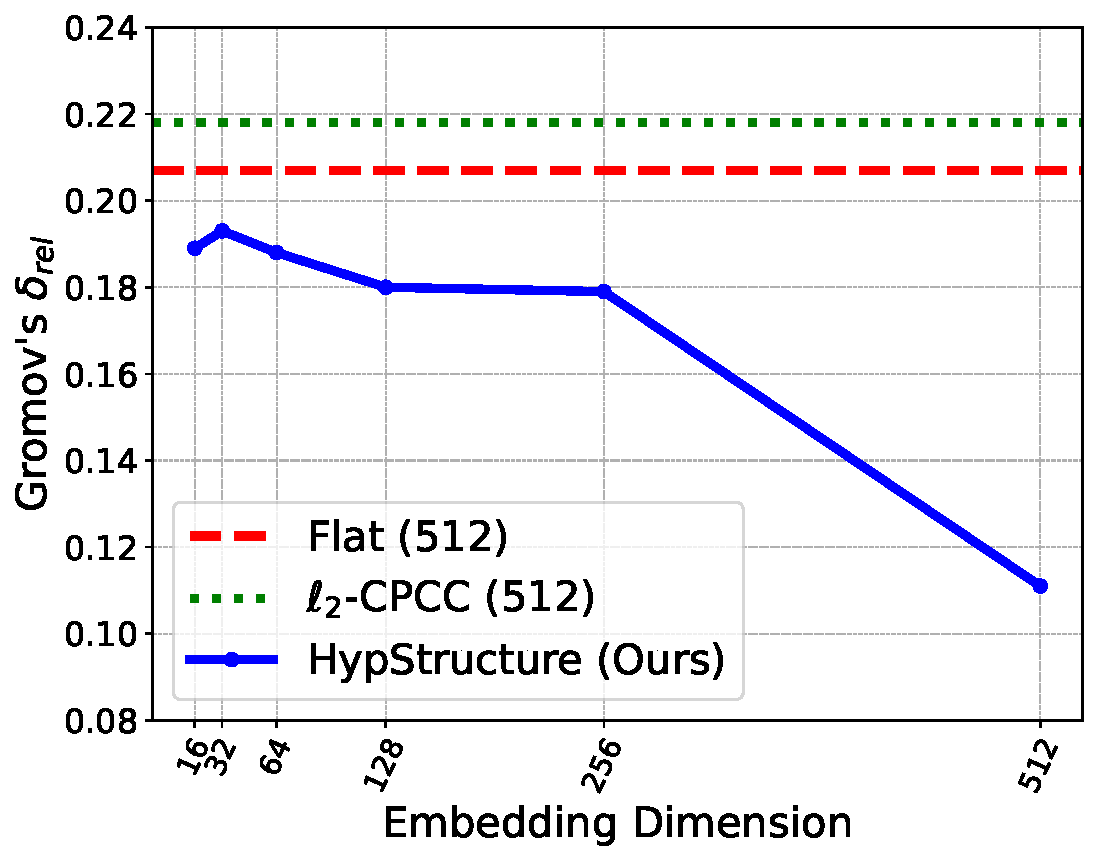
\includegraphics[width=\textwidth]{figures/gromov_delta_hypstructure_12.pdf}
        \caption{Evaluation of distortion vs feature dimensions for \texttt{HypStructure}.}
        \label{fig:gromov_delta}
    \end{minipage}
\end{figure*}

First, to assess the \emph{tree-likeness} of the learnt representations, we measure the Gromov's hyperbolicity $\delta_{rel}$ \citep{gromov1987hyperbolic, adcock2013tree, jonckheere2008scaled, khrulkov2020hyperbolic} of the features in \Cref{tab:combined_metrics_accuracy}. Lower $\delta_{rel}$ indicates higher tree-likeness and a perfect tree metric space has $\delta_{rel}=0$ (more details in \Cref{app:sec_delta_hyperbolicity}). To also evaluate the correspondence of the feature distances with ground truth tree metrics, we compute CPCC on test sets. We observe that \texttt{HypStructure} reduces distortion of hierarchical information over Flat by upto \textbf{59.4\%} and over $\ell_2$-CPCC by upto \textbf{45.4\%}, while also consistently improving the test CPCC for most datasets. 

We also perform a qualitative analysis of the learnt representations from \texttt{HypStructure} on the CIFAR10 dataset, and visualize them in a \Poincare disk using UMAP \citep{mcinnes2018umap} in \Cref{fig:hyp_umap_cifar10}. We can observe clearly that the samples for fine classes arrange themselves in the \Poincare disk based on the hierarchy tree as seen in \Cref{fig:toy}, being closer to the classes which share a \emph{coarse} class parent.

To examine the impact of feature dimension on the representative capacity of the hyperbolic space, we vary the feature dimension for \texttt{HypStructure} and compute the $\delta_{rel}$ for each learnt feature. Comparing the distortion of features with the Flat and $\ell_2$-CPCC settings in \Cref{fig:gromov_delta},  we observe that $\delta_{rel}$ decreases consistently with increasing dimensions, implying that high dimension features using \texttt{HypStructure} are more tree-like, and better than Flat and $\ell_2$-CPCCs' $512$-dimension baselines.

\begin{figure}[!ht]
    \centering
    \begin{minipage}{0.25\textwidth}
        \centering
        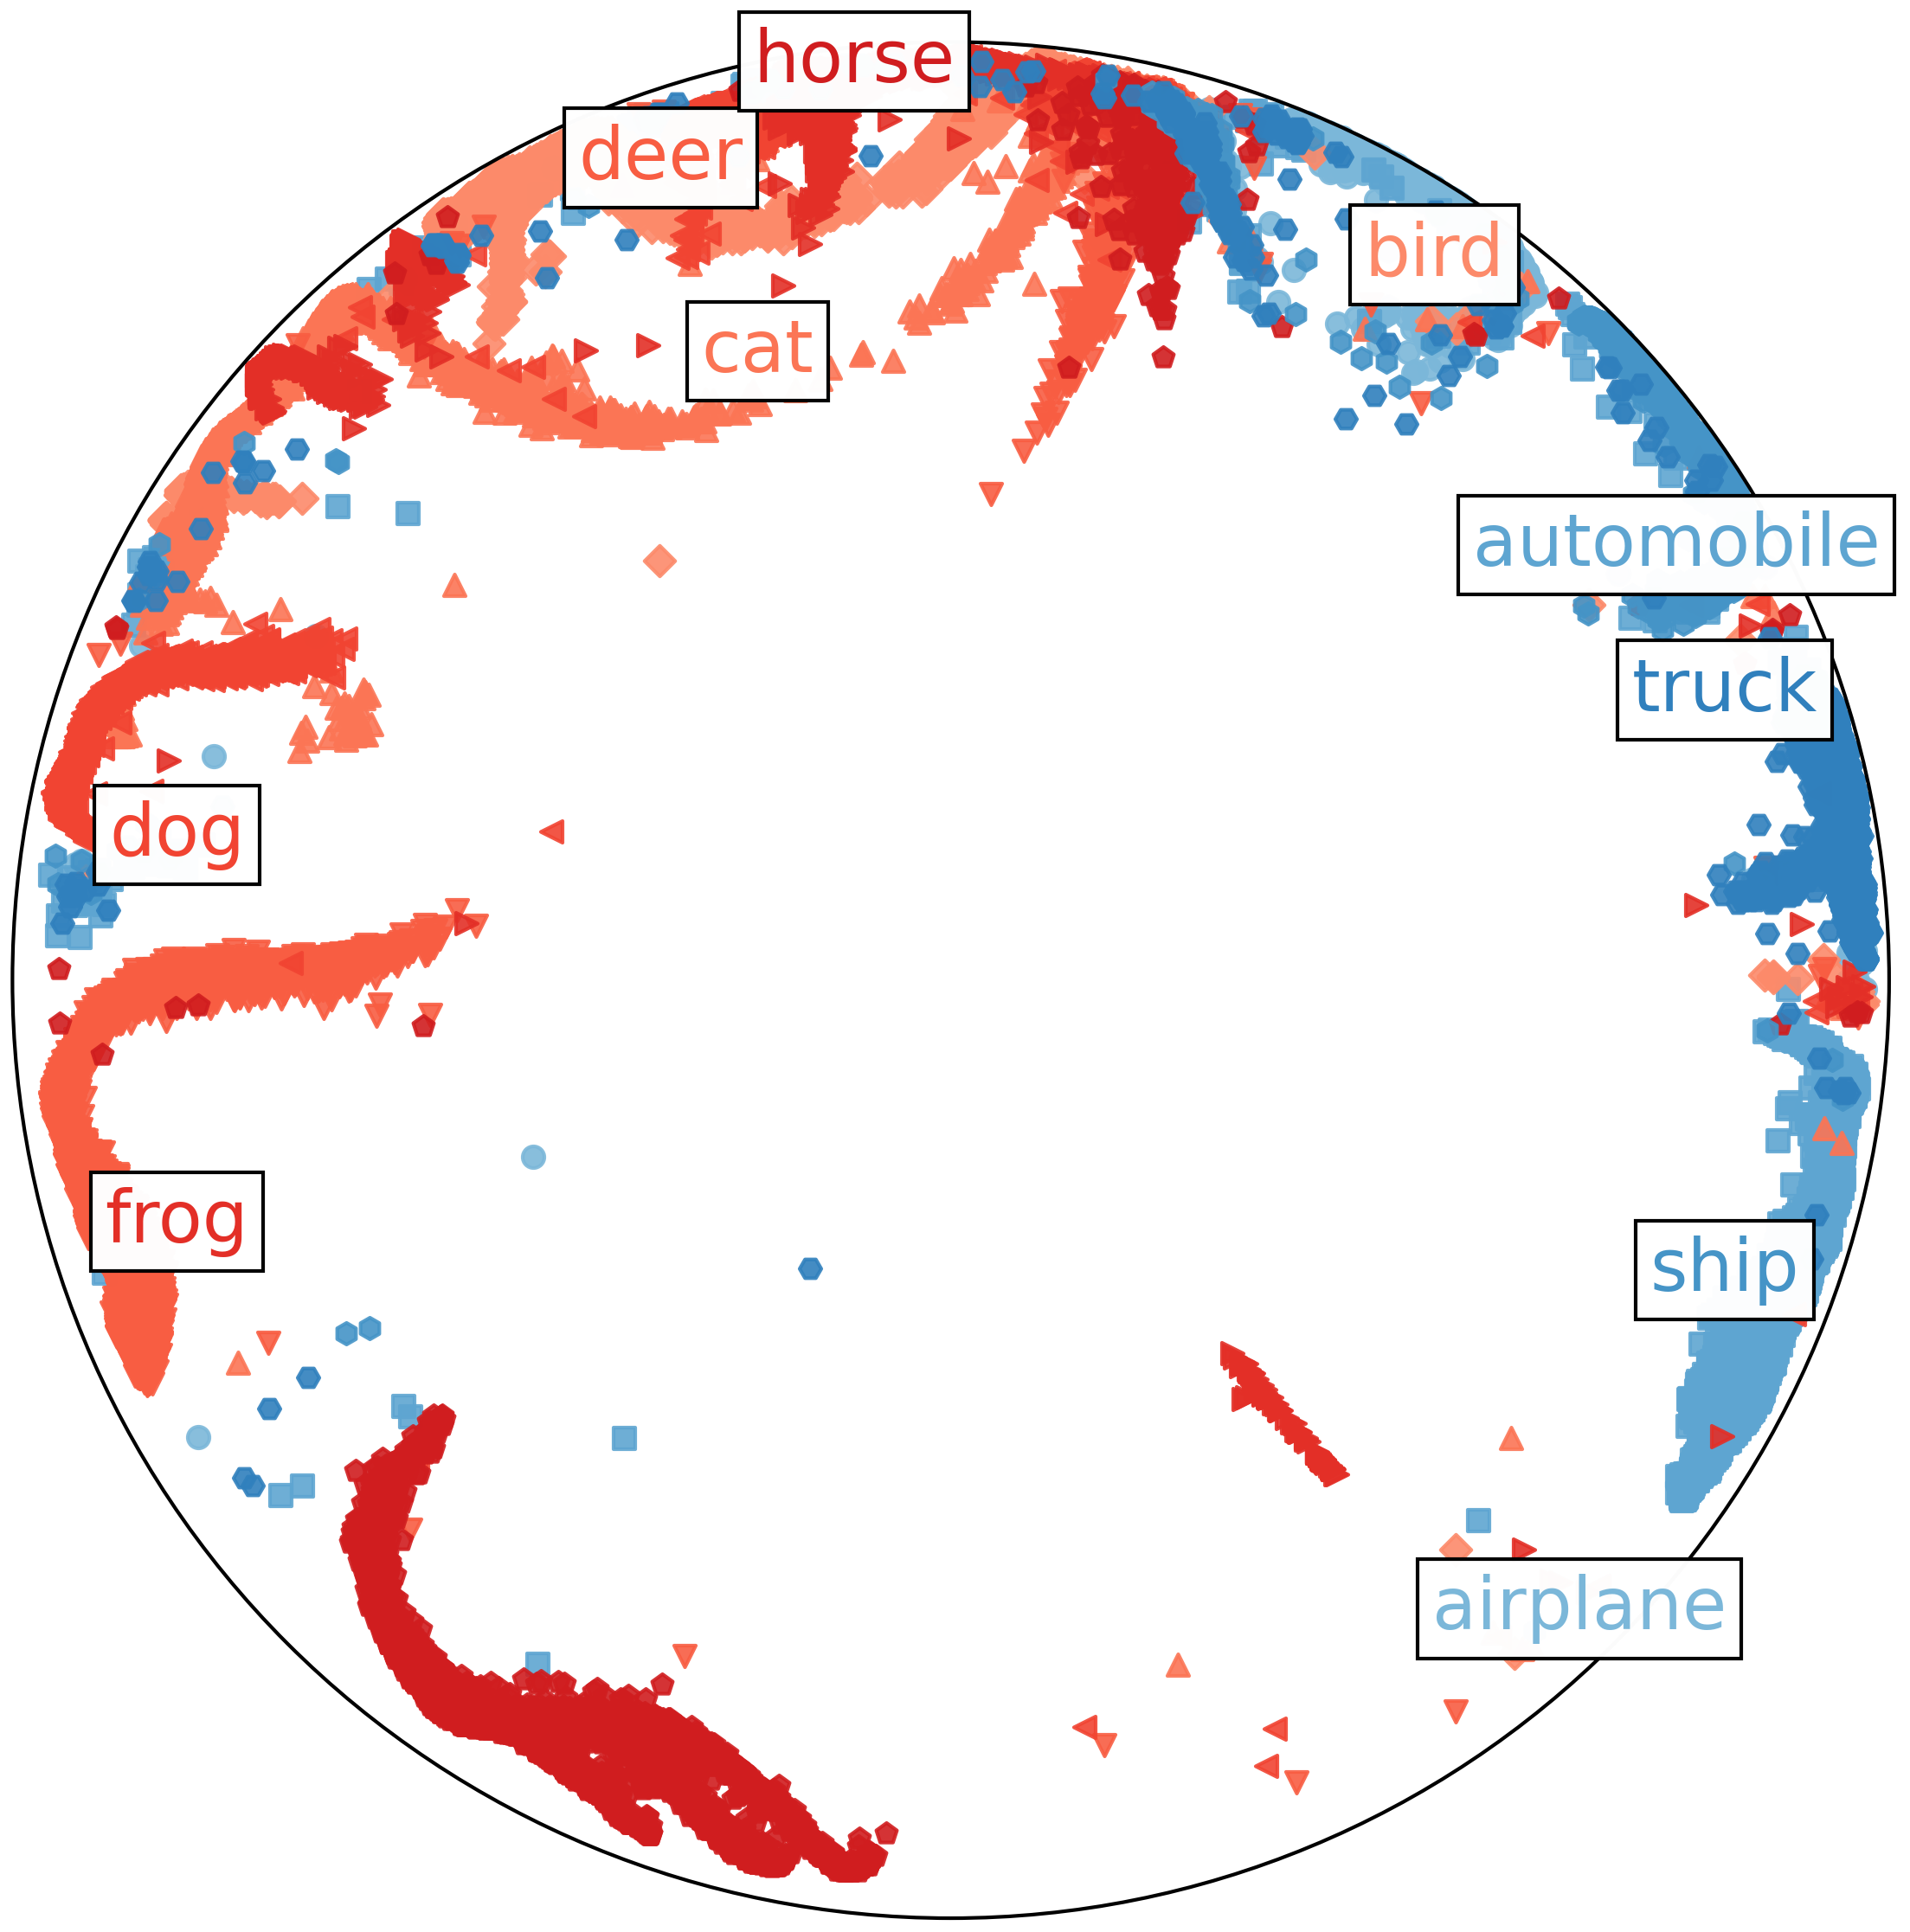
\includegraphics[width=\linewidth]{figures/hypstructure_cifar10_centers_main_1.png}
        \subcaption{\centering Hyperbolic UMAP: \texttt{HypStructure}}
        \label{fig:hyp_umap_cifar10}
    \end{minipage}
    \hfill
    \raisebox{5pt}{\begin{minipage}{0.32\textwidth}
        \centering
        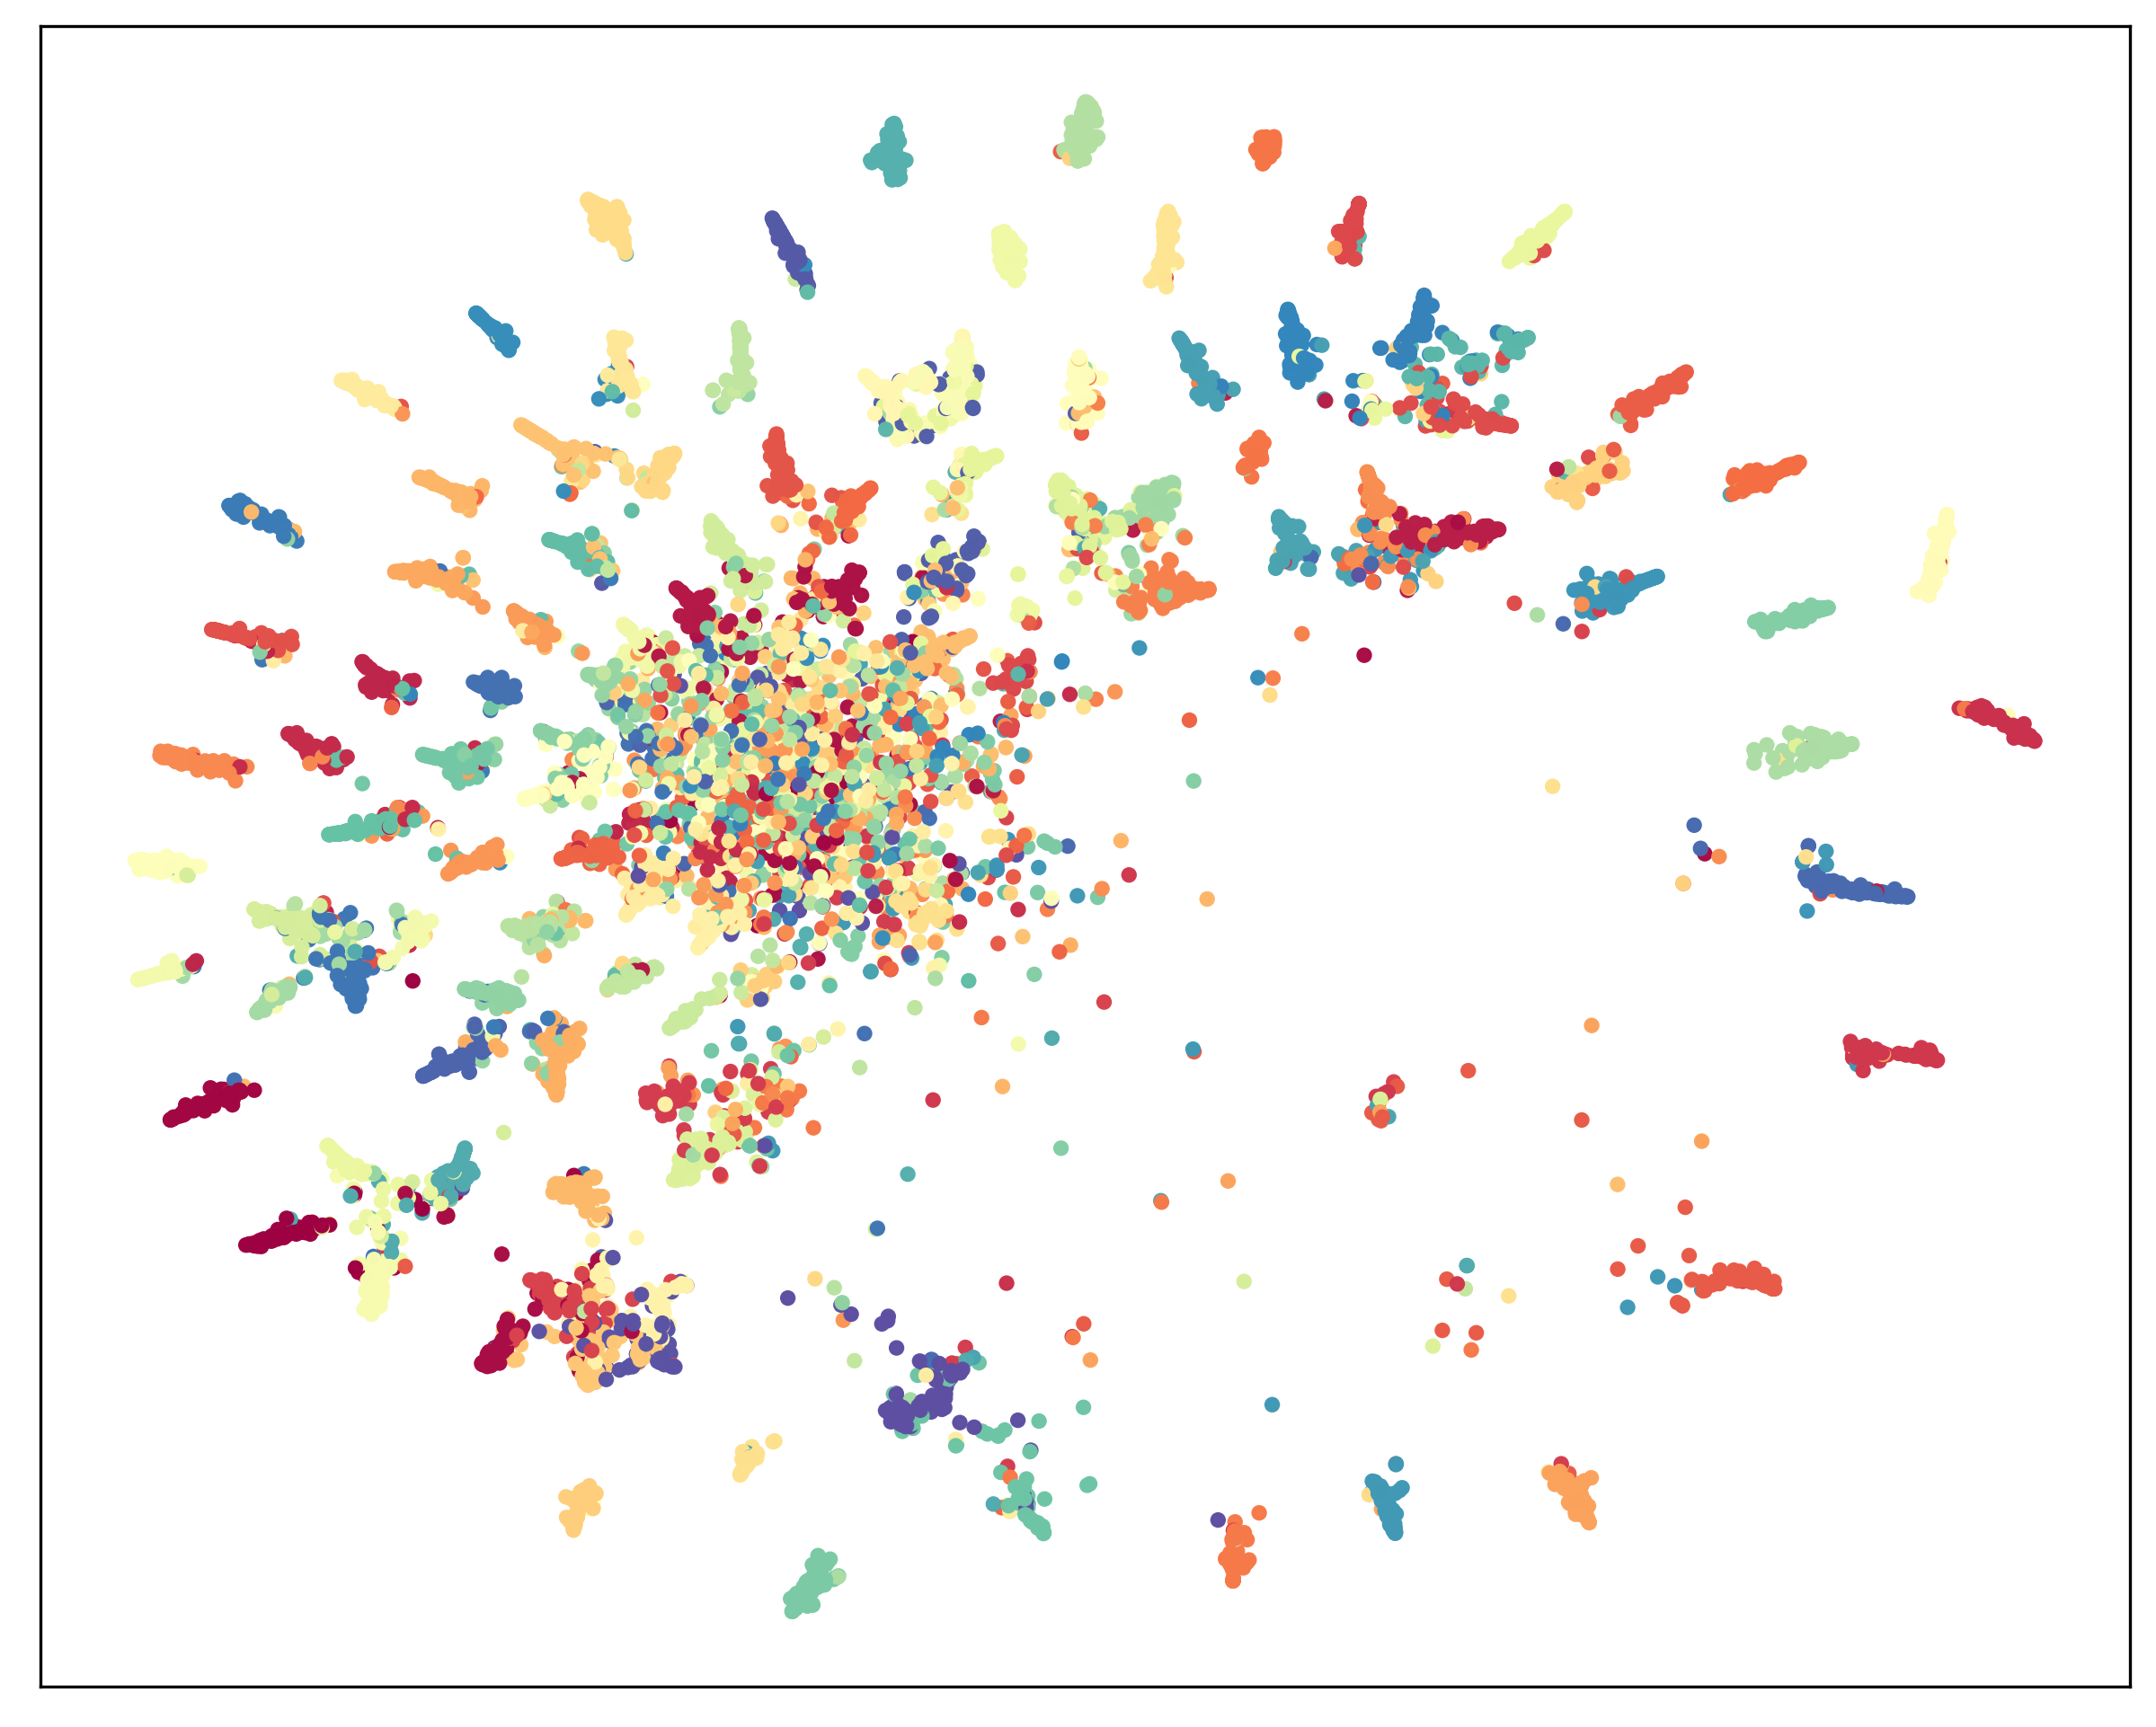
\includegraphics[width=\linewidth]{figures/supcon_base_cifar100_tsne_1.png}
        \subcaption{\centering Euclidean t-SNE: Flat}
        \label{fig:tsneflat}
    \end{minipage}}
    \hfill
    \begin{minipage}{0.32\textwidth}
        \centering
        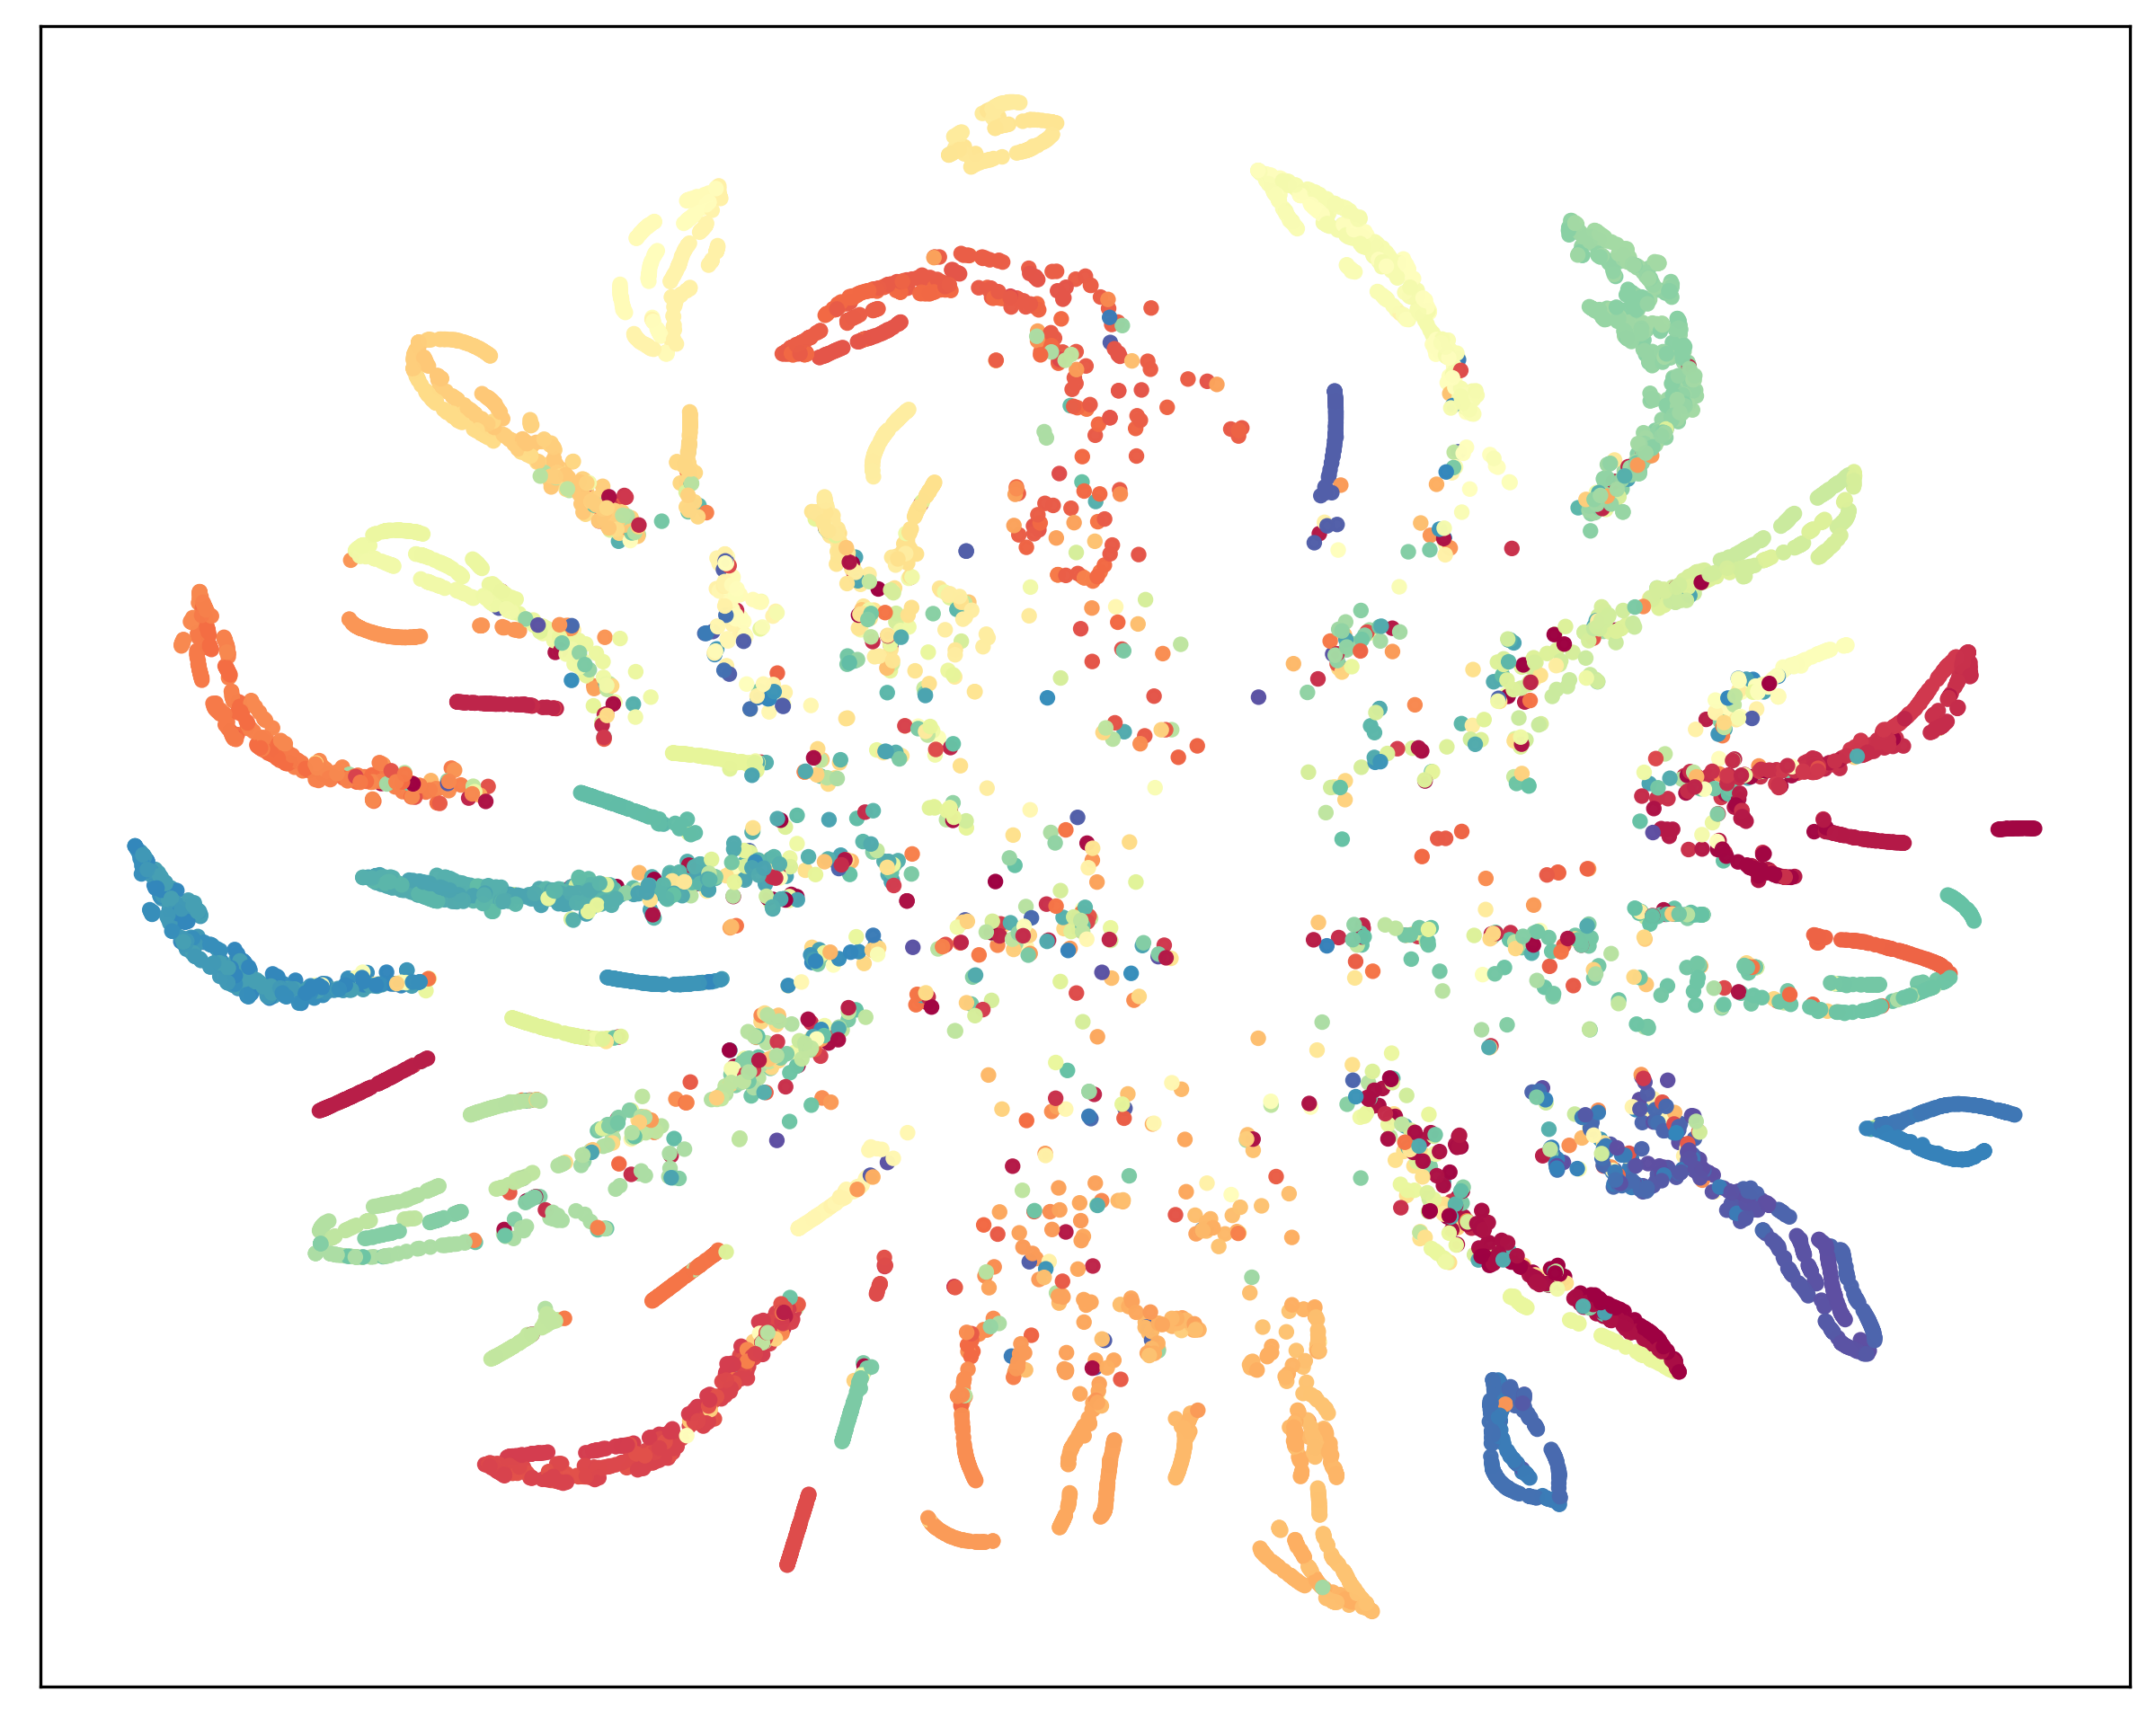
\includegraphics[width=\linewidth]{figures/hypstructure_cifar100_tsne_1.png}
        \subcaption{\centering Euclidean t-SNE: \texttt{HypStructure}}
        \label{fig:tsne_hypstructure}
    \end{minipage}
    \captionof{figure}{Left: Hyperbolic UMAP visualization of CIFAR10's \texttt{HypStructure} representation on \Poincare disk. Middle and Right: t-SNE visualization of learnt representations on CIFAR100.}
\end{figure}




\subsection{Classification}
Following \citet{zeng2022learning}, we treat leaf nodes in the hierarchy as \emph{fine} classes and their parent nodes as \emph{coarse} classes. To evaluate the quality of the learnt representations, we perform a classification task on the fine and coarse classes using a kNN-classifier following \citep{he2020momentum, wu2018unsupervised, caron2020unsupervised, zhuang2019local} and report the performance on the three datasets in \Cref{tab:combined_metrics_accuracy}. We observe that \texttt{HypStructure} leads to upto \textbf{2.2\%} improvements over Flat and upto \textbf{0.8\%} improvements over $\ell_2$-CPCC on both fine and coarse accuracy. We also visualize the learnt test features from Flat vs \texttt{HypStructure} on the CIFAR100 dataset using Euclidean t-SNE \citep{van2008visualizing} and show the visualizations in \Cref{fig:tsneflat} and \Cref{fig:tsne_hypstructure} respectively. We observe that \texttt{HypStructure} leads to sharper and more discriminative representations in Euclidean space. Additionally, we see that the fine classes belonging to a coarse class (the same shades of colors) which are semantically closer in the label hierarchy, are grouped closer and more compactly in the feature space as well, as compared to Flat. We also perform evaluations using the linear evaluation protocol \citep{2020supcon} and observe an identical trend in the accuracy, we report these results in \Cref{app:sec_linear_evaluation}.


\subsection{OOD Detection}
In addition to leveraging the hierarchy explicitly for the purpose of learning tree-like ID representations, we argue that a structured separation of features in the hyperbolic space as enforced by \texttt{HypStructure} is helpful for the OOD detection task as well. To verify our claim, we perform an exhaustive evaluation on 9 real-world OOD datasets and demonstrate that \texttt{HypStructure} leads to improvements in the OOD detection AUROC. We share more details below.

\begin{figure*}[h]
    \centering
    \begin{subfigure}[c]{0.75\textwidth}
        \centering
        \resizebox{\textwidth}{!}{
        \begin{tabular}{lcccccccccc}
        \toprule
        \multirow{2}{*}{\textbf{Method}} & \multicolumn{5}{c}{\textbf{OOD Dataset AUROC (↑)}} & \multicolumn{2}{c}{\textbf{Overall AUROC}} \\
        \cmidrule(lr){2-6} \cmidrule(lr){7-8}
        & SVHN & Textures & Places365 & LSUN & iSUN & \textbf{Avg.(↑)} & \textbf{B.C.(↑)} \\
        \midrule
        ProxyAnchor \citep{kim2020proxy} & 82.43 & 84.99 & 79.84 & 91.68 & 84.96 & 84.78 & 51.42 \\
        CE + SimCLR \citep{winkens2020contrastive} & 94.45 & 82.01 & 71.48 & 89.00 & 83.82 & 84.15 & 31.42 \\
        CSI \citep{tack2020csi} & 92.65 & 86.47 & 76.27 & 83.78 & \textbf{84.98} & 84.83 & 40.00 \\
        CIDER \citep{cider2022ming} & 95.16 & 90.42 & 73.43 & 96.33 & 82.98 & 87.67 & 60.00 \\
        \midrule
        SSD+ (\texttt{SupCon}) \citep{2021ssd} & 94.19 & 86.18 & \textbf{79.90} & 85.18 & 84.08 & 85.90 & 54.28 \\
        KNN+ (\texttt{SupCon}) \citep{sun2022knnood} & 92.78 & 88.35 & 77.58 & 89.30 & 82.69 & 86.14 & 40.00 \\
        $\ell_2$-CPCC \citep{zeng2022learning} & 93.08 & \textbf{90.45} & 77.21 & 82.77 & 82.79 & 85.26 & 40.00 \\
        \rowcolor{gray!20}\texttt{HypStructure} &  \textbf{95.97} & 88.43 & 78.12 & \textbf{97.01} & 84.51 & \textbf{88.81} & \textbf{82.85} \\
        \bottomrule
        \end{tabular}
        }
        \caption{OOD detection performance with CIFAR100 as ID dataset.}
        \label{tab:ood_detection_main_cifar100}
    \end{subfigure}
    \hfill
    \begin{subfigure}[c]{0.21\textwidth}
        \centering
        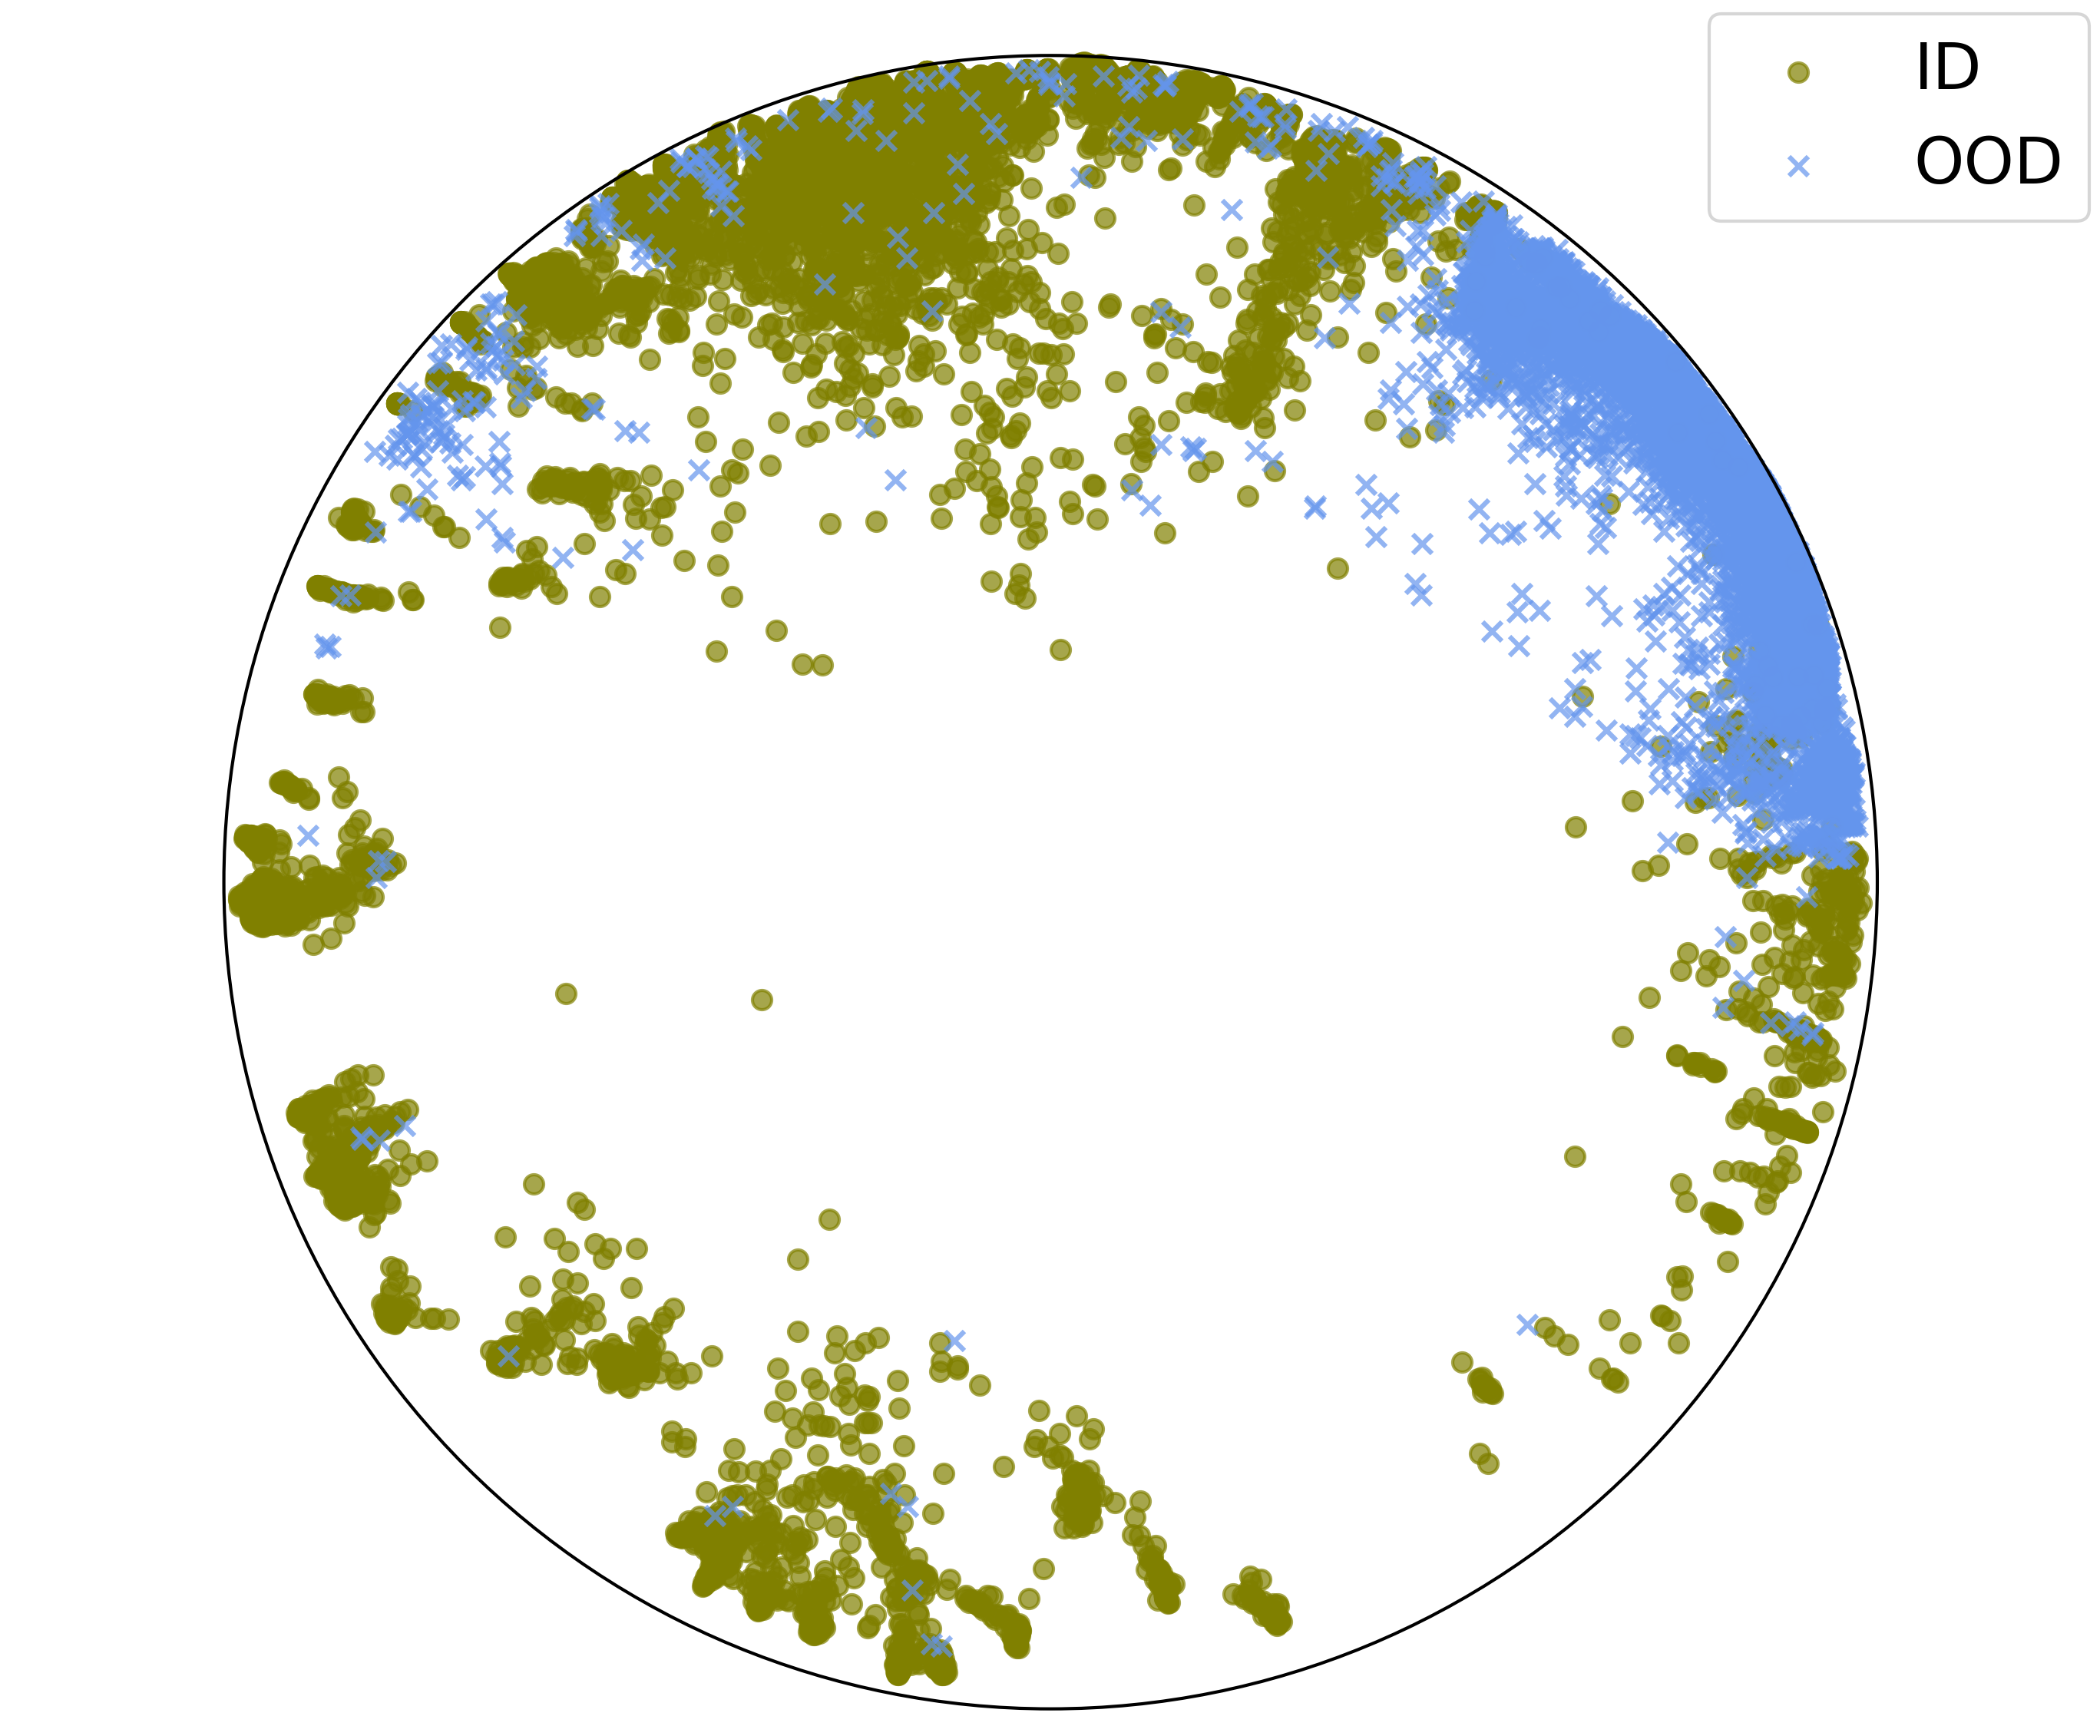
\includegraphics[width=\textwidth]{figures/hypstructure_poincare_disk_ID_OOD_1.png}
        \hspace{1pt}
        \caption{CIFAR100 (ID) vs. SVHN (OOD).}
        \label{fig:ood_viz}
    \end{subfigure}
    \caption{Left: OOD detection score across various datasets on the CIFAR100 ID dataset. Right: Hyperbolic UMAP of the CIFAR100 (ID) test vs SVHN (OOD) test features learnt from \texttt{HypStructure} with a clear separation in the \Poincare disk. }
\end{figure*}

\subsubsection{Problem Setting}

Out-of-distribution (OOD) data refers to samples that do not belong to the in-distribution (ID) and whose label set is disjoint from $\mathcal{Y}^{\text{in}}$ and therefore should not be predicted by the model. Therefore the goal of the OOD detection task is to design a methodology that can solve a binary problem of whether an incoming sample $\vx \in \mathcal{X}$ is from $P_{\mathcal{X}}$ i.e. $\*y \in \mathcal{Y}^{\text{in}}$ (ID)  or $\*y \notin \mathcal{Y}^{\text{in}}$ (OOD).


\textbf{OOD datasets} We evaluate on 5 OOD image datasets when CIFAR10 and CIFAR100 are used as the ID datasets, namely \texttt{SVHN}~\citep{svhn}, \texttt{Places365}~\citep{zhou2017places}, \texttt{Textures}~\citep{texture}, \texttt{LSUN} ~\citep{lsun}, and \texttt{iSUN}~\citep{isun}, and 4 large scale OOD test datasets, specifically \texttt{SUN} \citep{lsun}, \texttt{Places365} \citep{zhou2017places}, \texttt{Textures} \citep{texture} and \texttt{iNaturalist} \citep{Horn_2018_CVPR} when ImageNet100 is used as the ID dataset. This subset of datasets is prepared by \citep{ming2022delving} and is created with overlapping classes from ImageNet-1k removed from these datasets to ensure there is no overlap in the distributions.

\textbf{OOD detection scores}
While several scores have been proposed for the task of OOD detection, we evaluate our proposed method using the Mahalanobis score \citep{2021ssd}, computed by estimating the mean and covariance of the in-distribution training features. The Mahalanobis score is defined as
\begin{equation}
    s(\vx) = (f(\vx) - \mu)^\top\Sigma^{-1}(f(\vx) - \mu),
    \label{eq:mahalanobis}
\end{equation}
where $\mu, \Sigma$ are the mean and covariance of in-distribution training features. \citet{2021ssd} present the Mahalanobis score (\cref{eq:mahalanobis}) in a generalized version for multiple feature clusters. However, since they empirically observe that the single-cluster version achieves the highest performance \citep{2021ssd}, we will focus on this version.

After computing the OOD detection scores, we measure the area under the receiver operating characteristic curve (AUROC) as the primary evaluation metric following \citet{lee2018simple, 2021ssd}. 




\subsubsection{Main Results and Discussion}
\begin{table}[tb]
\centering
\caption{OOD detection AUROC with CIFAR10 and ImageNet100 as ID.}
\label{tab:ood_detection_cifar_imagenet}
\begin{tabular}{lc|lc}
    \toprule
    \textbf{Method} & \textbf{AUROC} & \textbf{Method} & \textbf{AUROC}\\
    \midrule
    \multicolumn{2}{c}{\textbf{CIFAR10}} & \multicolumn{2}{c}{\textbf{ImageNet100}} \\
    SSD+ & 97.38 & SSD+ & 92.46 \\
    KNN+ & 97.22 & KNN+ & 92.74 \\
    $\ell_2$-CPCC & 76.67 & $\ell_2$-CPCC & 91.33 \\
    \rowcolor{gray!20}\texttt{HypStructure} & \textbf{97.75} & \texttt{HypStructure} & \textbf{93.83}\\
    \bottomrule
\end{tabular}
\end{table}

We report the AUROC averaged over all the OOD datasets (5 datasets for CIFAR10 and CIFAR100, 4 datasets for ImageNet100) in \Cref{tab:ood_detection_main_cifar100} and \Cref{tab:ood_detection_cifar_imagenet} In addition to the Flat (\texttt{SupCon}) and $\ell_2$-CPCC baselines, we also compare our method with other state-of-the-art methods (see \Cref{app:ood_citations} for more details about existing OOD detection methods). We observe that \texttt{HypStructure} leads to a consistent improvement in the OOD detection score, with upto \textbf{2\%} in average AUROC. We also report the dataset-wise OOD detection results for the CIFAR100 ID dataset in Table \ref{tab:ood_detection_main_cifar100} along with Average AUROC. To remove the bias in the Average AUROC metric towards any single dataset, we also evaluate the Borda Count (B.C.) \citep{McLean_Urken_Hewitt_1995} and report the same, along with a detailed comparison with more OOD detection methods in Table \ref{tab:ood_detection_main_cifar100}, 
and Tables \ref{tab:main_c10_ood} and \ref{tab:main_im10_ood} in the \Cref{app:sec_ood_detection}.

We observe that \texttt{HypStructure} ranks in the highest performing methods consistently, thereby demonstrating a higher Borda Count as well. We additionally visualize the CIFAR100 (ID) vs SVHN (OOD) features learnt from \texttt{HypStructure}, using a hyperbolic UMAP visualization in \Cref{fig:ood_viz}. We observe that training with \texttt{HypStructure} leads to an improvement in the separation of ID vs OOD features in the \Poincare disk. 

\textbf{Additional Experiments,  Ablations and Visualizations:} More experiments using hyperbolic contrastive losses and hyperbolic networks, ablation studies on each component of \texttt{HypStructure} and additional visualizations can be found in \Cref{app:secC}.

\section{Eigenspectrum Analysis of Structured Representations}
\label{sec:eigenspectrum_theory}

\begin{figure}[ht]
    \centering
    \raisebox{8pt}{\begin{subfigure}[c]{0.25\textwidth}
        \centering
    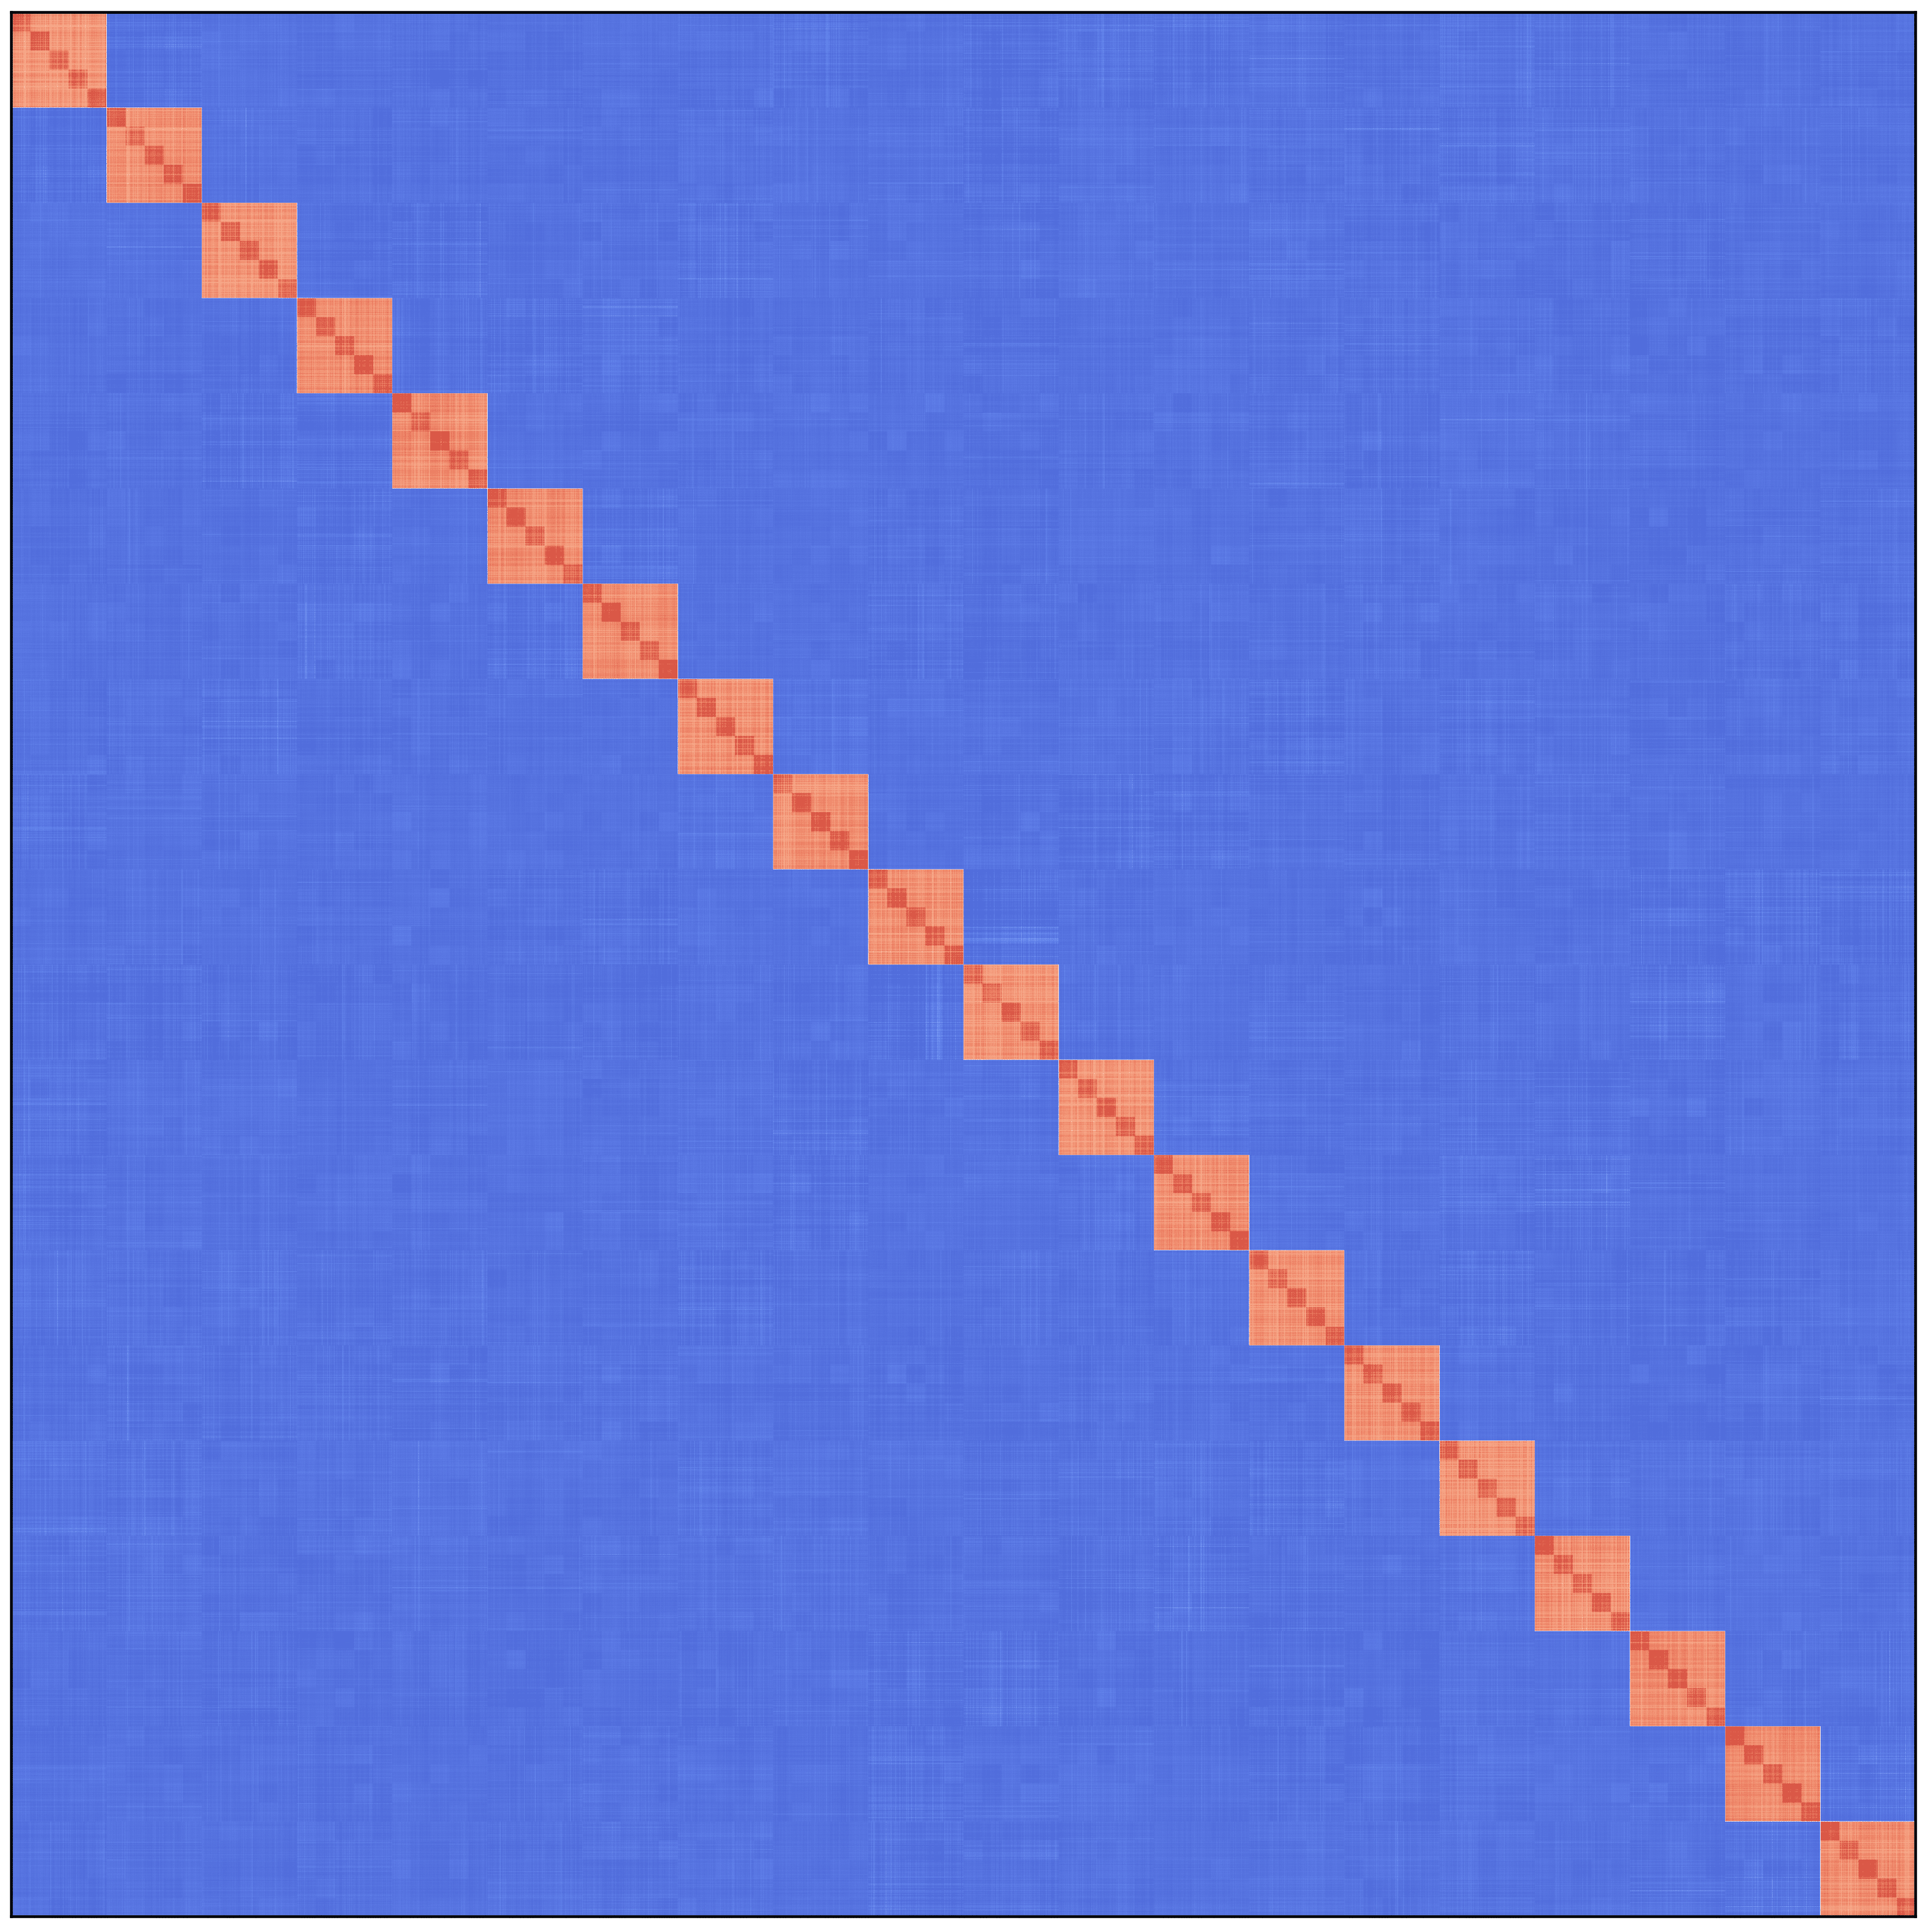
\includegraphics[width=\textwidth]{figures/poincare-matrix.png}
    \phantomsubcaption
    \label{fig:poincare-matrix}
    \end{subfigure}
    }
    \hfill
    \begin{subfigure}[c]{0.32\textwidth}
        \centering
        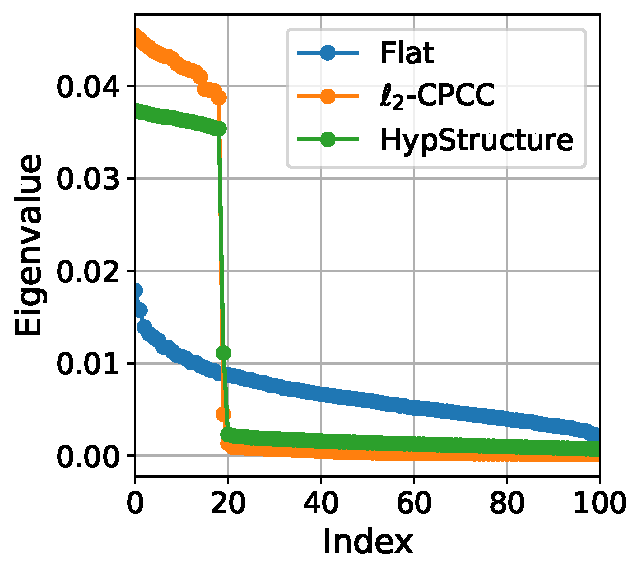
\includegraphics[width=\textwidth]{figures/eigenspectrum.pdf}
        \phantomsubcaption
        \label{fig:eigenspectrum}
    \end{subfigure}
    \hfill
    \raisebox{-3pt}{\begin{subfigure}[c]{0.4\textwidth}
        \centering
        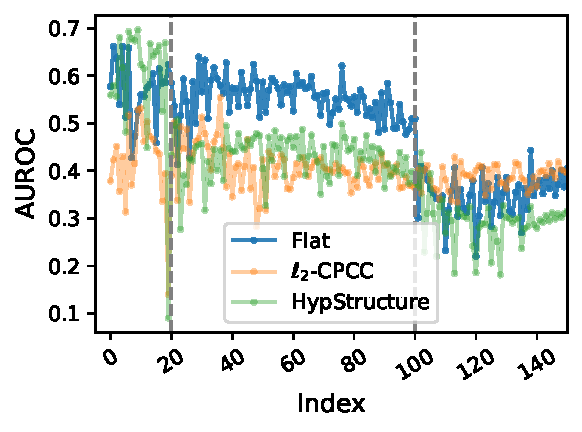
\includegraphics[width=\textwidth]{figures/CIFAR100SVHN.pdf}
        \phantomsubcaption
        \label{fig:CIFAR100SVHN}
    \end{subfigure}
    }
    \vspace{-10pt}
    \caption{CIFAR100 as in-distribution dataset. Left (a): Hierarchical block pattern of $K$. Middle (b): Top 100 eigenvalues of $K$ for different representation. Right (c): OOD detection for CIFAR100 vs. SVHN with the top $k$-th principal component.}
    \label{fig:three_figures}
\end{figure}


As seen in \Cref{tab:ood_detection_main_cifar100}, we observe a significant improvement in the OOD detection performance using \texttt{HypStructure} with the Mahalanobis score \cref{eq:mahalanobis}. After training a composite loss with CPCC till convergence, let us denote the matrix of the normalized in-distribution trained feature as $Z \in \mathbb{R}^{n \times d}$. Naturally, we inspect the eigenvalue properties of $\Sigma$ (i.e, $Z$), and observe that $K = ZZ^\top \in \mathbb{R}^{n \times n}$ exhibits a hierarchical block structure (\Cref{fig:poincare-matrix}) where the diagonal blocks have a significantly higher correlation than other off-diagonal values, leading us to the following theorem.  

\begin{restatable}[\textbf{Eigenspectrum of Structured Representation with Balanced Label Tree}]{theorem}{balanced}
    \label{thm:eigen} 
      \textit{Let $\mathcal{T}$ be a balanced tree with height $H$, such that each level has $C_h$ nodes, $h \in [0,H]$. Let us denote each entry of $K$ as $r^h$ where $h$ is the height of the lowest common ancestor of the row and the column sample. If $r^h \geq 0, \forall h$, then:  (i) For $h = 0$, we have $C_0 - C_1$ eigenvalues $\lambda_0 = 1 - r^1$. (ii) For $0 < h \leq H-1$, we have $C_{h} - C_{h+1}$ eigenvalues $\lambda_h = \lambda_{h-1} + (r^{h} - r^{h+1})\frac{C_0}{C_h}$. (iii) The last eigenvalue is $\lambda_{H} = \lambda_{H-1} + C_0 r^H$.}
\end{restatable}

We defer the eigenspectrum analysis for an arbitrary label tree to \Cref{app:sec_proof}. \Cref{thm:eigen} implies a \textbf{phase transition pattern} in the eigenspectrum. There always exists a significant gap in the eigenvalues representing each level of nodes in the hierarchy, and the eigenvalues corresponding to the coarsest level are the highest in magnitude. CIFAR100 has a balanced three-level label hierarchy where each coarse label has five fine labels as its children. In \Cref{fig:eigenspectrum}, we visualize the eigenspectrum of CIFAR100 for \texttt{HypStructure}, $\ell_2$-CPCC and the Flat objective. We observe a significant drop in the eigenvalues for features learnt from two hierarchical regularization approaches, $\ell_2$-CPCC and \texttt{HypStructure}, at approximately the 20\textsuperscript{th} largest eigenvector (which corresponds to the number of coarse classes), whereas these phase transitions do not appear for standard flat features. We also observe that the magnitude of coarse eigenvalues are approximately at the same scale. 

In summary, \Cref{thm:eigen} helps us to formally characterize the difference between flat and structured representations. CPCC style (\cref{eq:CPCC}) regularization methods can also be treated as dimensionality reduction techniques, where the structured features can be explained mostly by the coarser level features. For the OOD detection setting, this property differentiates the ID and OOD samples at the coarse level itself using a lower number of dimensions, and makes the OOD detection task easier. We visualize the OOD detection AUROC on SVHN (OOD) corresponding to the CIFAR100 (ID) features with the top$-k$ principal component for different methods, in \Cref{fig:CIFAR100SVHN}. We observe that for features learnt using \texttt{HypStructure}, accurately embedding the hierarchical information leads to the top $20$ eigenvectors (corresponding to the coarse classes) being the most informative for OOD detection. Recall that CIDER \citep{cider2022ming} is a state-of-the-art method proposed specifically for improving OOD detection by increasing inter-class dispersion and intra-class compactness. We note that CPCC style (\cref{eq:CPCC}) methods can be seen as a generalization of CIDER on higher-level concepts, where the same rules are applied for coarse labels as well, along with the fine classes. When the ID and OOD distributions are far enough, using coarse level feature might be sufficient for OOD detection.